\documentclass{article}

\usepackage{authblk}
\title{Supplementary Methods, Tables, and Figures}
 \author[1]{Wancen Mu}
 \author[2]{Eric S. Davis}
 \author[5]{Stuart Lee}
 \author[6]{Mikhail G. Dozmorov}
 \author[2,3]{Douglas H. Phanstiel}
 \author[1,4]{Michael I. Love \thanks{michaelisaiahlove@gmail.com}}
 \affil[1]{Department of Biostatistics, }
 \affil[2]{Curriculum in Bioinformatics and Computational Biology, }
 \affil[3]{Thurston Arthritis Research Center, Department of Cell Biology \& Physiology, Lineberger Comprehensive Cancer Center, Curriculum in Genetics \& Molecular Biology, and}
 \affil[4]{Department of Genetics, University of North Carolina-Chapel Hill, NC 27599}
 \affil[5]{Genentech, South San Francisco, CA, USA}
 \affil[6]{Department of Biostatistics, Department of Pathology, Virginia Commonwealth University, Richmond, VA 23298, USA}

\date{\today}
\usepackage{graphicx}
\usepackage{graphics}
\usepackage{amsmath}
\usepackage{threeparttable}
\usepackage[top=1in,left=1in,right=1in,bottom=1in]{geometry}
\usepackage[usenames,dvipsnames,svgnames,table]{xcolor}
\usepackage{xspace}
% \usepackage{hyperref}
\usepackage[colorlinks=true,linkcolor=black,citecolor=blue,urlcolor=blue,]{hyperref}
\usepackage{natbib}
\usepackage{xcite}
\usepackage{courier}

% cross-ref with main paper
\usepackage{xr}
\makeatletter
\newcommand*{\addFileDependency}[1]{% argument=file name and extension
  \typeout{(#1)}
  \@addtofilelist{#1}
  \IfFileExists{#1}{}{\typeout{No file #1.}}
}
\makeatother
\newcommand*{\myexternaldocument}[1]{%
    \externaldocument{#1}%
    \addFileDependency{#1.tex}%
    \addFileDependency{#1.aux}%
}
\myexternaldocument{plain}


\usepackage[ruled,vlined,linesnumbered,noresetcount]{algorithm2e}

\newcommand\mycommfont[1]{\footnotesize\ttfamily\textcolor{blue}{#1}}
\SetCommentSty{mycommfont}
\usepackage{float}
\usepackage[section]{placeins}
\usepackage[capitalise,noabbrev]{cleveref}
\usepackage{stfloats}
\usepackage{bm}
\usepackage{booktabs}
\usepackage{diagbox} % for diag line in table
\usepackage{hyperref}
\usepackage{geometry}
\usepackage{bm}
\usepackage{amsfonts,amssymb} %font
\usepackage{amsthm}
\usepackage{booktabs}
\usepackage{subfigure}
\geometry{a4paper,scale=0.8}
\renewcommand{\thefigure}{S\arabic{figure}}
\renewcommand{\thetable}{S\arabic{table}}
\renewcommand{\thesubfigure}{\Alph{subfigure}}

\usepackage[utf8x]{inputenc} % deal with "-" not usually set up by the [utf8] option

\newcommand{\code}[1]{\texttt{#1}}
\newcommand{\bootranges}{\emph{bootRanges}\xspace}
\newcommand{\nullranges}{\emph{nullRanges}\xspace}
\newcommand{\granges}{\texttt{GRanges}\xspace}
\newcommand{\plyranges}{\emph{plyranges}\xspace}
\newcommand{\mike}[1]{\textcolor{red}{[Mike: #1]}}
\newcommand{\wancen}[1]{\textcolor{purple}{[wancen: #1]}}


\usepackage{listings}
\lstset{basicstyle=\footnotesize\ttfamily}
\lstset{numbers=left, %设置行号位置
        numberstyle=\tiny, %设置行号大小
        keywordstyle=\color{blue}, %设置关键字颜色
        commentstyle=\color[cmyk]{1,0,1,0}, %设置注释颜色
        frame=single, %设置边框格式
        escapeinside=``, %逃逸字符(1左面的键),用于显示中文
        %breaklines, %自动折行
        extendedchars=false, %解决代码跨页时,章节标题,页眉等汉字不显示的问题
        xleftmargin=1em,xrightmargin=1em, aboveskip=1em, %设置边距
        tabsize=4, %设置tab空格数
        showspaces=false %不显示空格
       }
\usepackage{xcolor}

% \geometry{a4paper,left=2cm,right=2cm,top=1cm,bottom=1cm}

\begin{document}

\maketitle

\section{Supplementary Methods}\label{sec:suppmethods}

\subsection{Comparison to previous methods}

In order to generate background ranges for hypothesis
testing of association analysis, there are two general categories of methods.  
One strategy is to sample from a larger experimental pool or
database.
Methods following this strategy include
LOLA \citep{sheffield2016lola} using Fisher's exact test, 
Poly-Enrich \citep{lee2020poly} using a likelihood ratio test based on
a Negative Binomial likelihood, and matchRanges
\citep{Davis2022matchranges}
utilizing a covariate-based matching method.
Another strategy is to permute or shuffle the genomic ranges, possibly considering an
exclusion list of regions where the original region set should not be
re-located. Example methods belonging to this category include
bedtools shuffleBed \citep{quinlan2010bedtools}, ChIP-Enrich
\citep{welch2014chip}, and
GenometriCorr \citep{GenometriCorrfavorov2012}.
In addition, the method GAT allows controlling for GC content \citep{GAT_2013},
and regioneR implements a circular shift to
preserve the clumping property of genomic ranges \citep{gel2016regioner}.
Our method falls in the second category in that we redistribute
ranges along the genome, though we use a block resampling scheme 
to preserve local genome structure, as proposed for genomic region sets by
\citet{bickel2010subsampling}.

\subsection{Segmentation}

In the following, we define genome segmentation and how it pertains to
block bootstrap resampling, as proposed by \citet{bickel2010subsampling}.
The overall motivation for bootstrapping with respect to a segmented
genome is to preserve large scale genomic structure, e.g. large
regions with low or high density of genomic features such as
genes. This preservation of structure through segmentation is in
addition to the preservation of local clumping property of ranges, which is
accomplished by resampling blocks.

In this work, we segmented the genome based on gene density. We
downloaded the Ensembl v86 genes \citep{ensemblTrimmedEntry} 
%\wancen{should we use this reference instead? \citep{EnsDb.Hsapiens.v86}}, 
and counted the 
number of genes per million base pairs. We then supplied this vector
of counts to various methods for segmentation. We sought to define
sections of the genome that exhibit stationarity, where in this case,
stationary means similar gene density within a segment. We
additionally sought to group together segments across the genome that
had similar gene density, such that a segmentation state
$i \in [1,\dots,S]$ consisted of one or more non-contiguous regions of
the genome with similar gene density.

For block bootstrapping with respect to genome segmentations,
we considered various genome segmentation methods,
Circular Binary Search (CBS) \citep{cbs} and a hidden Markov model (HMM)
\citep{rcpphmm}, as well as pre-defined segmentations,
ChromHMM applied to 
Roadmap Epigenomics data \citep{ernst2012chromhmm}.
CBS and HMM
have R package implementations, and so we incorporated these
into a utility function in \nullranges, \texttt{segmentDensity()}.
CBS, implemented in the \textit{DNAcopy} package, was used to recursively split
chromosomes into subsegments with similar density. In this case, the
process was based on the square root of gene count per megabase to
stabilize variance and reduce the heavy right tail of the
distribution. We then used k-means to cluster
chromosome subsegments into groups with similar gene
density. We found that it was effective to cluster genome segmentations into
three states, corresponding to low, medium, and high gene
density. 
HMM was used to model the genes per megabase as an emission
density with pre-defined number of states. We found that three provided effective segmentation. 
We then used the Viterbi algorithm for the hidden state decoding. 
Roadmap segmentations derived by ChromHMM \citep{ernst2012chromhmm} were
downloaded from
\url{https://egg2.wustl.edu/roadmap/web_portal/}. ChromHMM is based on
a multivariate Hidden Markov Model that explicitly models the presence
or absence of many chromatin marks. The original ChromHMM annotation
generated segmentation including 
15 small states. We then summarized these into 3 general categories: low
density(`E9',`E13',`E14',`E15'), middle density(`E10',`E11',`E12'),
and high density(`E1-E8'). 
After merging, our version of ChromHMM applied to Roadmap data had
8,797 ranges were left and the mean width was around 
0.33 Mb.

\subsection{Simple region shuffling}\label{sec:shuffle}

Simple region shuffling was performed by placing ranges of interest
uniformly in acceptance regions with probability proportional to the
original SNP count per chromosome. For the paper, we defined
acceptance regions as the inverse of
ENCODE excluded regions \citep{amemiya2019encode},
centromeres, and telomeres from UCSC,
as provided in the \code{excluderanges} Bioconductor package
\citep{excluderanges}.

\subsection{Assessment of significance via bootstrap}

Suppose we are interested in computing and assessing the significance
of the overlap between one set of ranges
$\bm{x}$ and another set of ranges $\bm{y}$.
We compute the overlap $s_{obs}$, i.e. the total number of 
ranges in $\bm{x}$ that overlapped a range in $\bm{y}$.
This statistic can vary in many ways, including computing the fraction of
basepair overlap, restricting by a minimal amount of overlap, and
allowing for a gap between the ranges, e.g. we may allow 1 kb of gap
to connect local chromatin accessibility peaks to transcription start
sites (TSS).
Via block bootstrap resampling, we generate $R$ new
sets of ranges $\bm{y_r}$ within $R_b = R \times \sum_{c=1}^{C} ceiling(L_c / L_b)$ blocks, for the chromosome $c$ length $L_c$.
For details see \cref{alg:unseg} and \cref{alg:seg}.
We can perform either genome-wise, block-wise, or region-wise analysis
based on the question to be addressed. For example, if we want to test
the significance of the genome-wide amount of overlap, we would compare
to the genome-wise distribution. However, if we want to
test the significance of the number of overlaps for a particular
block or even a particular region, we could use a lower $R$ as there
will be many more bootstrapped blocks and bootstrapped ranges for a
block-wise or region-wise analysis.
Without loss of generality, we will consider the genome-wise case.
We use the overlaps per bootstrap sample $\bm{y_r}$ to calculate the
overlap statistics $s_{1}, s_{2}, \dots, s_{R}$
to derive a genome-wise empirical \textit{p}-value
$= \frac{1}{R} \sum_{r=1}^R \mathbb{I}_{\{s_r > s_\text{obs}\}}$ or
$s_{1}, s_{2},..., s_{R_b}$ for block-wise analysis.
Alternatively, we could use $z$ score to measure the
distance between $s_{obs}$ and the
set of $\{s_r\}$ in terms of standard deviations (SD).
Specifically, the
$z$ score in \cref{fig:result} is calculated by

$$ z = \frac{s_{obs} - \bar{s}}{ \text{SD}_R },$$

where
$\bar{s} = \frac{1}{R} \sum_{r=1}^R s_r$
is the sample mean of the overlap statistic $s_r$ over the $R$
bootstrap samples and 
$\text{SD}_R = \sqrt{\frac{1}{R-1} \sum_{r=1}^R [s_r - \bar{s}]^2}$ is
the sample standard deviation. 
Note that, if block-wise analysis is preferred as in
\citet{bickel2010subsampling}, we found out the SD of block-wise
bootstrap distribution should be approximately scaled by $\sqrt{L_b}$
in simulation in order to make genome-wise and block-wise $z$ score
comparative. In theory, the $\bar{s}$ is approximately the same in
both analyses, but the SD is different. As $\text{SD}_R$ captures
genome-wise SD, then block-wise SD is
$\text{SD}_{R_b} = \sqrt{\frac{1}{R_b-1} \sum_{r=1}^{R_b} [s_r - \bar{s}]^2} \approx \sqrt{\frac{L_b}{L_G}} \times \sqrt{\frac{1}{R}\sum_{r=1}^{R_b} [s_r - \bar{s}]^2}$,
for the whole genome length $L_G$.

\subsection{$L_b$ selection}\label{sec:length}

We considered two aspects of the block bootstrap datasets to select
block length $L_b$.
First, following \citet{bickel2010subsampling}, we tried to find $L_b$
that provided the minimum value of a pseudo-metric,

$$ d^*(v)= \left| \sqrt{\frac{L_{v-1}}{L_v}} [\text{IQR}(\mathcal{L}_{L_v})-\text{IQR}(\mathcal{L}_{L_{v-1}})] \right|,$$
where $\mathcal{L}_{L_v}$ is the distribution of the test statistic at
block length $L_v$, $v = 1,2,\dots,V$, $V$ is the number of candidate
block lengths, and $\text{IQR}(\mathcal{L})$ is the interquartile
range of a distribution $\mathcal{L}$.
Another aspect for block length selection is evaluating the
conservation of the spatial pattern. In order to provide robust
statistical inference in terms of significance testing,
the generated null models should have
similar spatial properties with 
the original sets, e.g. inter-range distances. Here we use
``null models'' interchangeably with block bootstrapped data.
We used the Earth's Mover
Distance (EMD) to quantify the similarity of the distributions of
inter-range distances between the original and null models, resulting 
in values from zero (identical distributions) to one (totally disjoint
distributions) \citep{emd}.
The EMD between two distributions is proportional to
the minimum amount of ``work'' required to change one distribution ($y$)
into the other ($y'$). Here $y$ and $y'$ are the histograms of
original and null model inter-range distance.
We observed that EMD always decreased as $L_b$ increased, because more
neighboring ranges' distances were preserved in the
block bootstrap with larger blocks (block boundaries break original
distances).
However, $L_b$ cannot be too large and close to $L_s$.
Otherwise, the randomization of blocks would not
be effective: the blocks will not sufficiently shuffle ranges across
segments within a particular segmentation state.
Hence, we decided an optimal $L_b$ falls in the range where EMD
was around elbow of the line plot for this aspect. 

\subsection{Block bootstrapping algorithm in \bootranges}\label{sec:algorithm}
\wancen{Segmentation with proportional length blocks are theoretical advantageous to accurate estimate null distribution (\citet{bickel2010subsampling}). However, in practice, if the segments are very heterogeneous in size, smaller size segments will construct too short blocks. When considering segmentation or un-segmented, segmentation are always preferred given the heterogeneity of large-scale genomic sequences. If the purpose is block bootstrapping on a small pieces of genomic, un-segmented algorithm may be sufficient. And \cite{bickel2010subsampling} have demonstrate the advantages of using segmentation by simulation. If un-segmented is considered to use, block bootstrap will be preferred over permutation as it better provides the uncertainty of the statistics distribution in the observed data by allowing repetitive resampling. }

\begin{algorithm}[H]
\SetNoFillComment
\caption{Un-segmented block bootstrap / permutation} \label{alg:unseg}  
\KwData{Ranges ($\bm{y}$), Block length ($L_b$), Length of
  chromosome $c$ ($L_c$), Total number of chromosomes ($C$),
  Bootstrap iterations ($R$), Type ($permute$ or $bootstrap$),
  Excluded regions ($\bm{e}$)}
\KwResult{$\texttt{BootRanges}$ object, with the bootstrapped
  region sets from each iteration, concatenated across $R$ total
  iterations. Iteration and $L_b$ recorded as metadata}
$r \gets 1$\\
\While{$r \leq R$}{
  \texttt{rearranged blocks} $\gets$ Generate consecutive tiling
  blocks with width $L_b$ (except last tile per chromosome which
  is cut to fit $L_c$ for chromosome $c$)\\
  \uIf{permutation}{
    \texttt{random blocks} $\gets$ Sample blocks without replacement from rearranged blocks
  }\ElseIf{bootstrap}{ 
    $n_b \gets \sum_{c=1}^{C} \text{ceiling}(L_c / L_b)$\\
    \texttt{random blocks} $\gets$ Sample $n_b$ blocks with
    replacement from the genome, where sampling probability per
    chromosome is proportional to $L_c$\\
  }
  \texttt{bootstrap[r]} $\gets$ Shift ranges in $\bm{y}$ that fall in the \texttt{random blocks} to their
  respective positions in the \texttt{rearranged blocks}, trimming applied to any
  ranges that extend past chromosome end or into excluded regions $\bm{e}$
}
Concatenate \texttt{bootstrap} ranges across iterations $r$\\
\end{algorithm}

\begin{algorithm}
\SetNoFillComment
\caption{Segmented block bootstrap with fixed or proportional block length}\label{alg:seg}
\KwData{Ranges ($\bm{y}$), Maximal block length ($L_b$), Length of genome ($L_G$),
  Bootstrap iterations ($R$), Type ($fixed$ or $proportional$),
  Segmentation states $\mathcal S$,
  Segmentation regions $\mathcal{A}_s$ (the set of all ranges
  belonging to state $s$), and with $L_a^s$ representing the width of region $a$
  in state $s$, Excluded regions ($\bm{e}$)}
\KwResult{$\texttt{BootRanges}$ object}
$r \gets 1$\\
\While{$r \leq R$}{
  \ForEach{segmentation state $s \in \mathcal{S}$}{
    $L_s \gets \sum_{a \in \mathcal{A}_s} L_a^s$ $\dots$ thus $L_G = \sum_{s \in \mathcal S} L_s$ \\
    \uIf{fixed}{
      $n_b^s \gets \sum_{a \in \mathcal{A}_s} \text{ceiling}(L_a^s / L_b)$ \\
    }\ElseIf{proportional}{
      $L_b^s \gets L_b \cdot L_s / L_G$ $\dots$ thus $L_b^s \le L_b$ and equal iff $\mathcal S \equiv \{s\}$\\
      $n_b^s \gets \sum_{a \in \mathcal{A}_s} \text{ceiling}(L_a^s / L_b^s)$ \\
    }
    \texttt{rearranged blocks[s]} $\gets$ Generate $n_b^s$ consecutive tiling blocks over $\mathcal{A}_s$ \\
    \texttt{random blocks[s]} $\gets$ Sample $n_b^s$ blocks with replacement from $\mathcal{A}_s$,
    where number of blocks per $a$ is proportional to $L_a^s$ \\
  }
  Concatenate \texttt{rearranged blocks} and \texttt{random blocks} across $s$\\
  \texttt{bootstrap[r]} $\gets$ Shift ranges in $\bm{y}$ as in Algorithm \ref{alg:unseg}
}
Concatenate \texttt{bootstrap} ranges across iterations $r$\\
\end{algorithm}

\section{Supplementary Results} \label{sec:results}

\subsection{Simulation} \label{sec:sim}
\wancen{A small window of chromosome 4 was selected as one ranges set $\bm{x}$. Then we make 50 ranges sets $\bm{y}s$ whose features located in clumps. The number of gene within each cluster $\sim poisson(5)$ and the start position is uniformly chosen within a relatively larger window. Therefore, we would expect there is no association between $\bm{x}$ and $\bm{y}$. In order to compare the accuracy of shuffling and block bootstrapping, we shuffled and block bootstrapped 50 times within a relatively larger window. One realization is shown in (\cref{fig:simulation} A). Two situations of interested statistics are considered. One is simply based on genomic location - total number of overlaps, another one is based on the metadata column of one ranges set - total score. We computed those statistics between $\bm{x}$ and simulated, shuffling, bootstrapping dataset across 50 iterations (\cref{fig:simulation} B, C). In both case, the distribution of statistics using simulated dataset are highly overlapped with block bootstrapping. While shuffling generate distribution of statistics with similar mean, but smaller variance. To access the accuracy, we take the right 5\% tail of shuffling and found out 26\% simulation distribution falls in it, which represent a high false positive rate(FPR). When we take the tight 5\% of bootstrapping, FPR is around 6\% that as we desired. Therefore, we conclude that shuffling will overestimate how unlikely the observed statistics is and lead to misinterpretation of enrichment.}

\subsection{Overlap analysis of liver ATAC-seq peaks with GWAS SNPs} \label{sec:liveratac}

1,872 SNPs were download from the NHGRI-EBI GWAS catalog
\citep{gwascatalog} on September 22, 2021. We only extracted single
nucleotide variants associated with ``total cholesterol''. Liver ATAC-seq peaks
\citep{CURRIN20211169} aggregated from 20 samples were downloaded from
the GEO accession: GSE164870. All the peaks here were filtered by FDR adjusted \textit{p}-value $\leq 0.05$.
Then, genomic coordinates of consensus peaks were converted from hg19 to
hg38 using \code{liftOver} to obtain 221,606 peaks.

Based on the $L_b$ selection criteria, we found that $d^*$ had
smaller values in most cases when $L_b \in [300kb,800kb]$
(\cref{fig:suppfig0}A). When quantify the similarity of the distributions of
inter-range distances between the original and 
null models using EMD, we derived the histograms of
original and
null model inter-range distance with bin size = 0.3 under various
$L_b$ and $L_s$ settings.
For this aspect, $L_b \in [200kb,600kb]$ was
shown to be a good range by visualization of density plot
(\cref{fig:suppfig0}B) and according to the elbow of the EMD statistic
(\cref{fig:suppfig0}C). Combining two aspects, we concluded that $[300kb,600kb]$ was a good range for block length.

\subsection{Enrichment analysis of macrophage ATAC-seq and gene expression}\label{sec:splines}

We used the differential results for RNA-seq and ATAC-seq as
described in the \textit{fluentGenomics} workflow \citep{lee2020fluent}, with
the original data from a human macrophage experiment by \citet{alasoo2018shared}.
The contrast of interest was interferon gamma (IFNg) treatment. Since the
transcriptomic response to IFNg stimulation may involve increased
transcription factor binding to \textit{cis}-regulatory elements near
genes, and as ATAC-seq captures the accessibility and activity at
these regions, \citet{lee2020fluent} hypothesized and demonstrated an
enrichment of differentially accessible (DA) ATAC-seq peaks near
differentially expressed (DE) genes. While \citet{lee2020fluent}
assessed significance by randomly sub-setting the non-DE genes and
re-computing overlap with DA peaks, here we considered the block
bootstrap for statistical significance.

When performing block bootstrap on the number of overlaps,
using $L_b = 500kb$ and $R = 100$,
we obtained empirical $\textit{p}$-value $=0$ and $z = -108.1$.
We therefore rejected the null hypothesis and concluded that there was
significant enrichment of DA peaks near DE genes.

For fitting the generalized penalized splines, we used the \code{gam} function in
the \code{mgcv} package \citep{mgcv2011wood} to fit the model, based on
a penalized likelihood maximization. Generalized cross-validation
was used to choose the optimal value for the smoothing parameter,
$\lambda$. Then, the \code{tidymv} package was used to predict and
extract the fitted value. 
For each generated null set, we found all the predicted overlap counts
for genes with logFC falling in the range (-8,10) with 1 as the
increment. Then, conditional density plots can be plotted across all
null sets. Additionally, we used a $z$ score to measure the distance of
predicted overlap counts between observed sets and the null sets in
terms of SD of the conditional null set (conditioning on logFC bin).

The following code shows how the analysis of Fig 2C is performed as
the downstream task following \bootranges. Suppose $x$ contains the DE genes and
$bootRanges$ contains the bootstrapped DA peaks. For each gene within each
iteration, we extract the total number of peaks that overlap with that
gene and that gene's logFC
(below, \texttt{max} is used to reduce a set
of repeated, identical values to a single numeric).
Then, after fitting splines, we predict
overlap counts for a 2,000 point grid spanning the original logFC range.
These spline-predicted values are those used to define the conditional
density.

\begin{lstlisting}[language=R]
boot_stats <- x %>% plyranges::join_overlap_inner(bootRanges) %>%
  plyranges::group_by(id.x, iter) %>%
  plyranges::summarize(count = plyranges::n(), logFC = max(x_logFC)) %>%
  as.data.frame() %>%
  tidyr::complete(`id.x`, iter, fill=list(count = 0)) %>%
  dplyr::select(iter, count, logFC) %>%
  tidyr::nest(-iter) %>%
  dplyr::mutate(
	 fit= map(data, ~gam(count ~ s(logFC), data = ., family=poisson)),
         pred  = map(fit, ~predict_gam(model = ., length_out = 2000)),
         fitted = map(pred, ~find_fit(data=., logFC = seq(-8,10,1))))

\end{lstlisting} 

\pagebreak

\subsection{Correlation analysis of Single Cell ATAC + Gene Expression}

We were interested in demonstrating \bootranges on data from single
cell experiments, in particular looking at correlations at
pseudo-bulk resolution in single cell multi-omics datasets.
For this purpose, 
data were downloaded from \citet{Vignette}, including
RNA-seq for genes and ATAC-seq for peaks in 10,032 cells.
Cell type annotations had already bee performed
by the 10x Genomics R\&D team. Information on genes and peaks from
chromosomes 1-22 were selected.
First, we aggregated data from cells within same cell type, to form
pseudo-bulks data with $n=14$ cell types according to the metadata. 
The pseudo-bulk data provided smoother correlation statistics without
loss of the information of interest (correlation of cell-type-specific
expression and accessibility).
Next, we removed all the ranges with 0
standard deviation in either assay.
Finally, log counts per million (CPM) were computed
from \code{edgeR} \citep{edgeR2010Robinson} to account for different library sizes
in both assays.

Our expectation was that the two modalities would have
significantly high correlation for peaks close to genes ($le 1kb$).
For the whole gene set, the mean
correlation of gene RNA-seq and peak ATAC-seq read counts was 0.33, while the
bootstrap sampling correlation distribution in \cref{fig:suppfig3}A
had a mean correlation of 0.007 for $R = 1,000$.
Therefore, as expected, RNA and ATAC
measured at nearby peaks had similar cell-type-specificity.
Additionally, the average gene-peaks correlation per gene can be
computed and compared to a bootstrap distribution to identify 5,644
gene-promoter pairs that were significantly correlated across cell
types. Among these, 5,591 genes had only one paired promoter, while 25
genes had 2 nearby promoters (peaks of accessibility within 1kb of the
body of a gene). 
%Those significant pairs could provide important insights into
%perturbation experiments for validation.
Two examples of the most significant gene-peak pairs are shown in
\cref{fig:suppfig3}B-C.

The following code is an example of how such an analysis can be
performed with \bootranges and \plyranges. Here $x$ refers to RNA-seq and $y$ refers to ATAC-seq.

\begin{lstlisting}[language=R]
# split count matrix into NumericList metadata and sort
x <- x_Granges %>%
  mutate(counts_X = NumericList(asplit(x.cpm, 1))) %>% sort()
y <- y_Granges %>%
  mutate(counts_y = NumericList(asplit(y.cpm, 1))) %>% sort()

# standardize read counts for fast correlation computation
x$counts_x <- NumericList(lapply(x$counts_X, function(z) (z-mean(z))/sd(z)))
y$counts_y <- NumericList(lapply(y$counts_y, function(z) (z-mean(z))/sd(z)))

# generate block bootstrap ranges for 'y'
boots <- bootRanges(y, blockLength = 5e5, R = 100)

# for standardized x and y:
correlation <- function(x,y) 1/(length(x)-1) * sum(x*y)

# extract bootstrap summary statistics
boot_stats <- x %>% plyranges::join_overlap_inner(boots, maxgap=1000) %>%
  plyranges::mutate(rho = correlation(counts_x, counts_y)) %>%
  plyranges::group_by(iter) %>%
  plyranges::summarise(meanCor = mean(rho)) 
\end{lstlisting} 
 
\newpage

\section{Supplementary Figures}

\begin{figure*}[htbp]
\centering
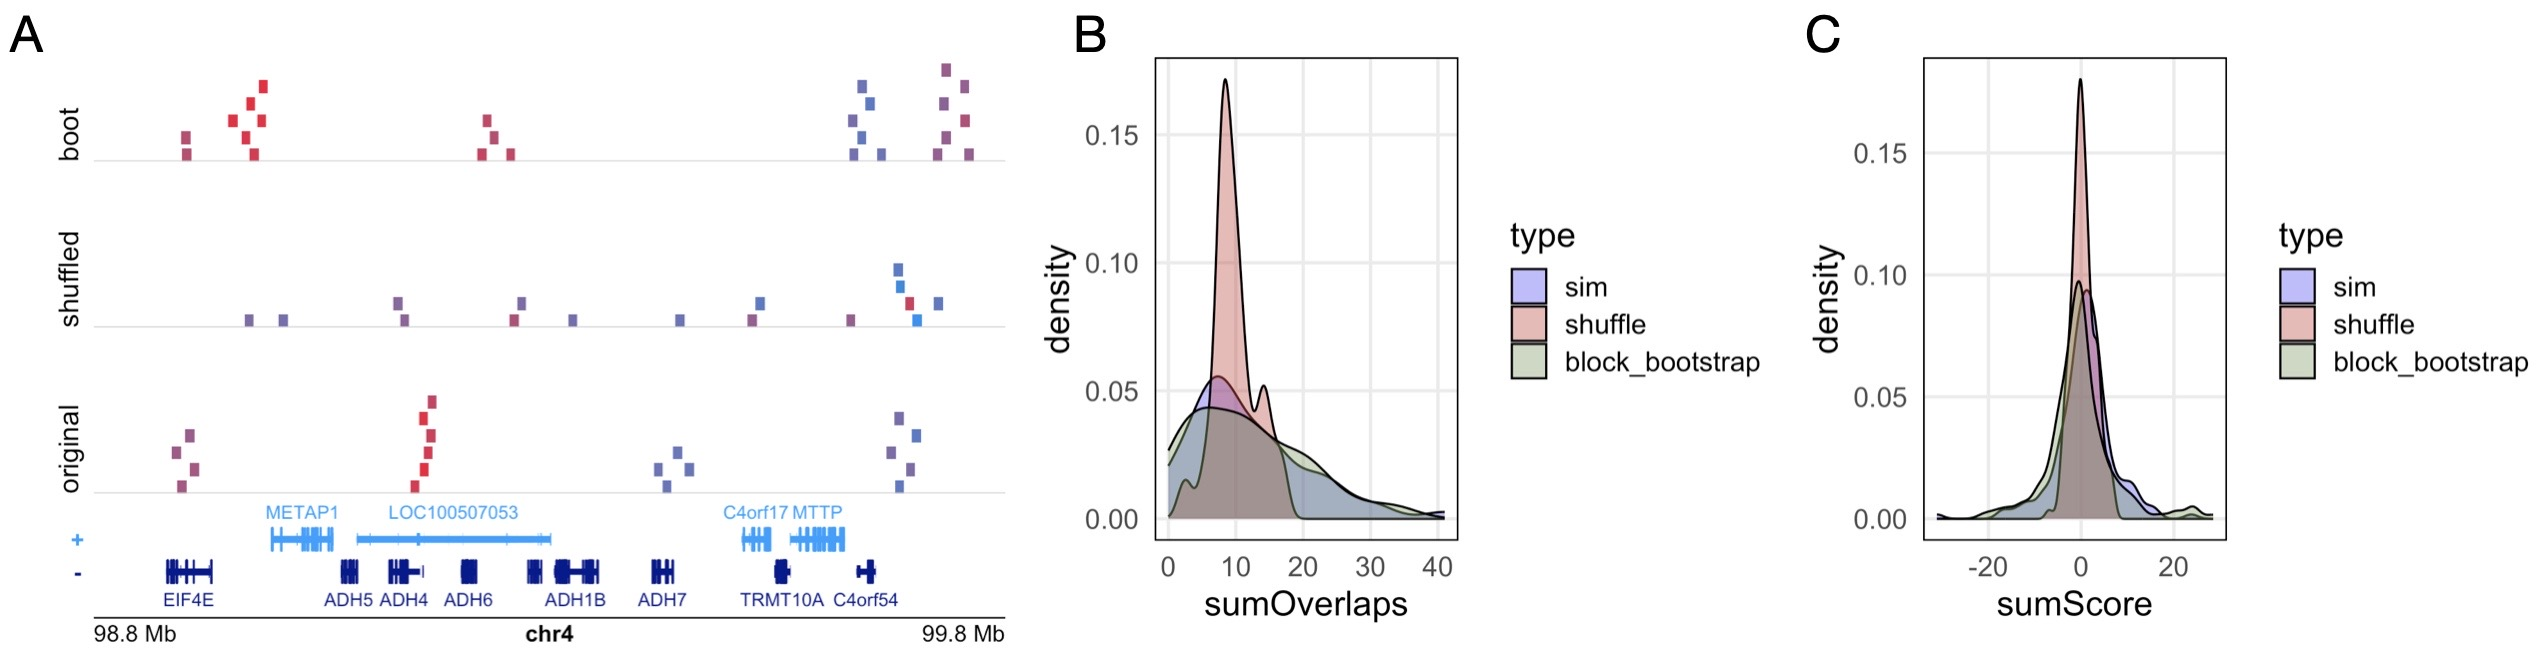
\includegraphics[scale=0.2]{Figures/simulation.jpg}
\caption{Comparison of shuffling and block bootstrapping in simulation. A) Visualization of one iteration of simulation. The bottom ranges set is $\bm{x}$, original is randomly simulated clustered range set $\bm{y}$. Shuffling does not preserve clumping properties on the genome, but bootstrapping keeps the local dependency. B) Density plots of total number of overlaps between $\bm{x}$ and simulated, shuffling, bootstrapping dataset across 50 iterations, respectively. C) Density plots of total scores in metadata column between $\bm{x}$ and simulated, shuffling, bootstrapping dataset across 50 iterations, respectively.}
\label{fig:simulation}
\end{figure*}

\begin{figure*}[htbp]
\centering
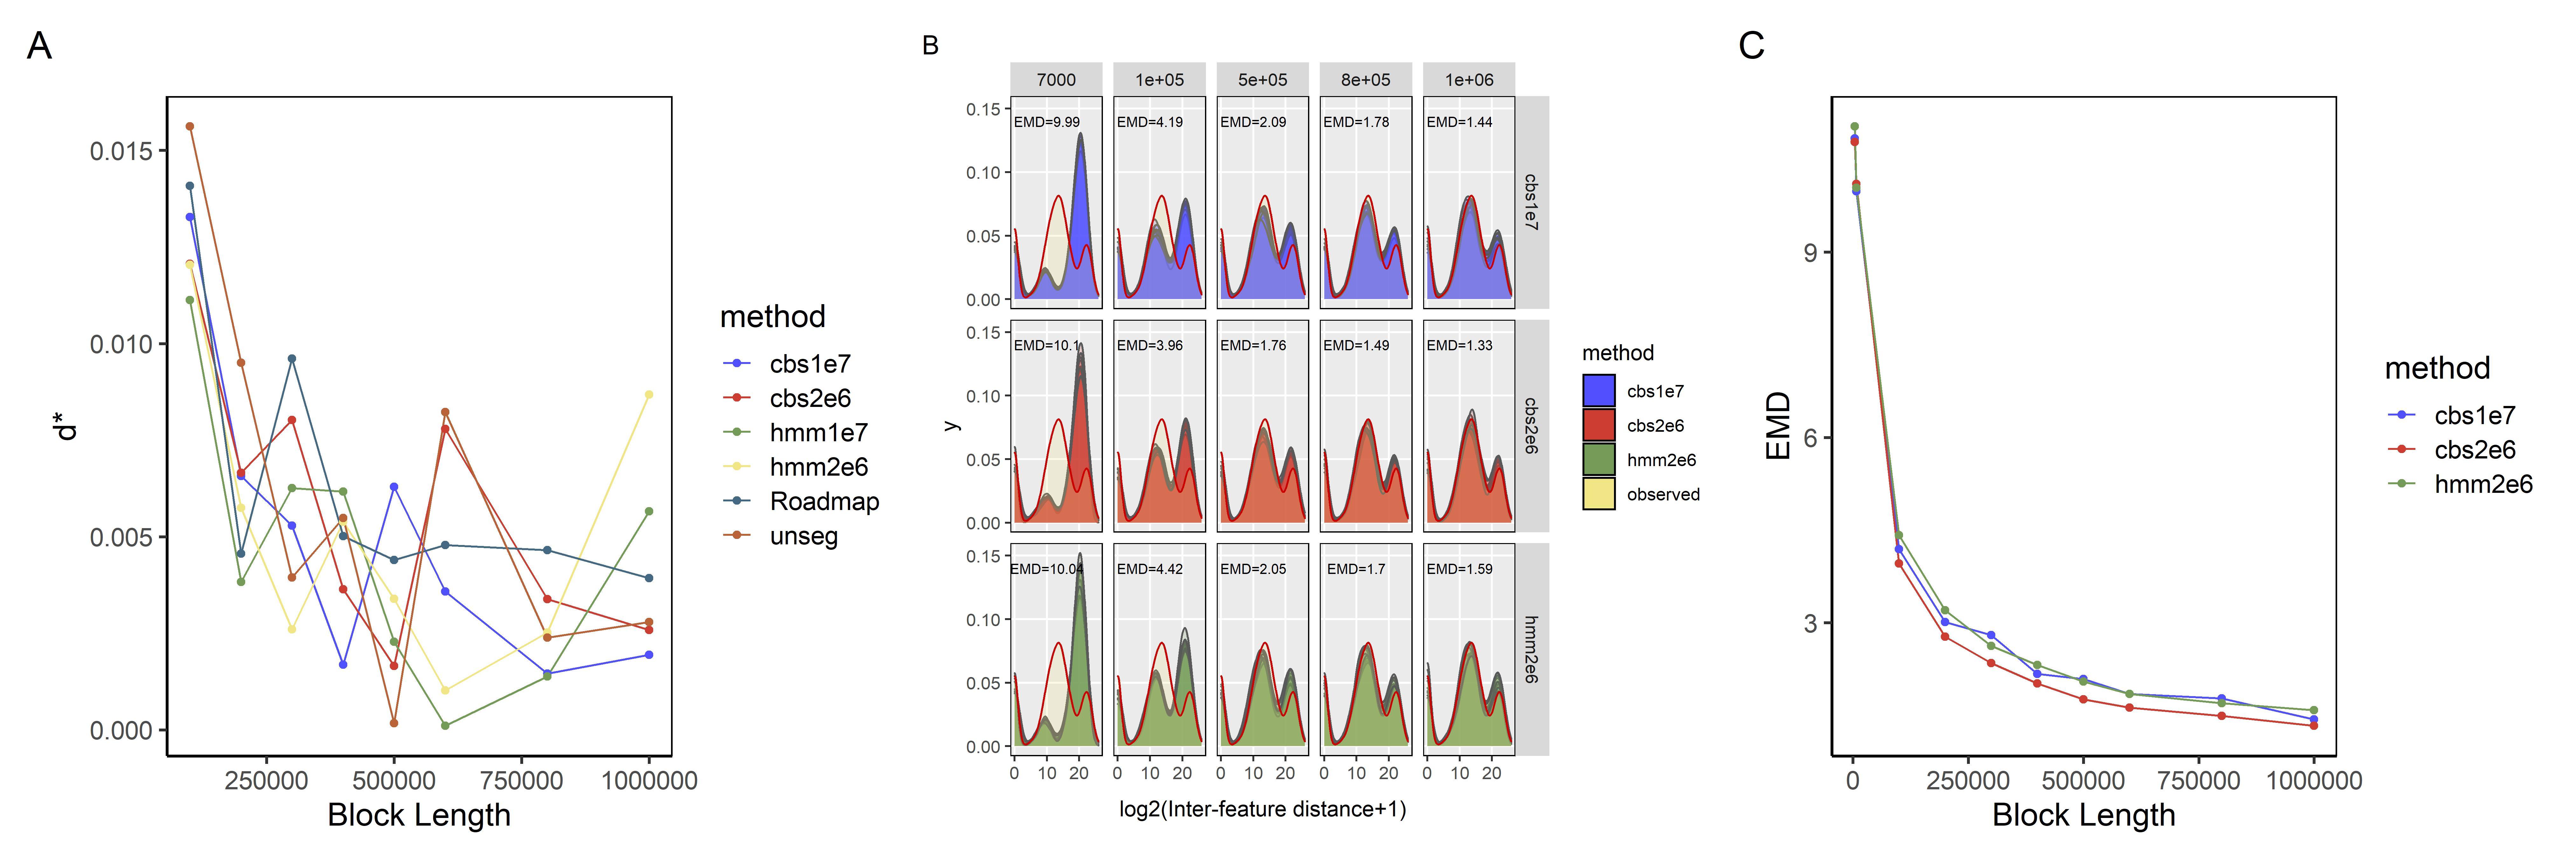
\includegraphics[scale=0.35]{Figures/sfig1.jpeg}
\caption{$L_b$ selection assessment. A) A pseudo-metric $d^*$
  \citep{bickel2010subsampling} over $L_b$ , B) 
  log2(inter-range distance+1) density plots over various $L_b$ and
  segmentation settings. Red curve represents the observed ranges'
  log2(inter-range distance+1) density.
  The more a particular null set's density
  plot overlapped with observed ranges, the better we conserved the
  spatial distribution of the original set via block
  bootstrapping. Median EMD shown as text in each panel. C) Median
  EMD over $L_b$ where EMD quantified the similarity of inter-range
  distance distributions between nulls sets and observed sets.}
\label{fig:suppfig0}
\end{figure*}

\begin{figure*}[htbp]
\centering
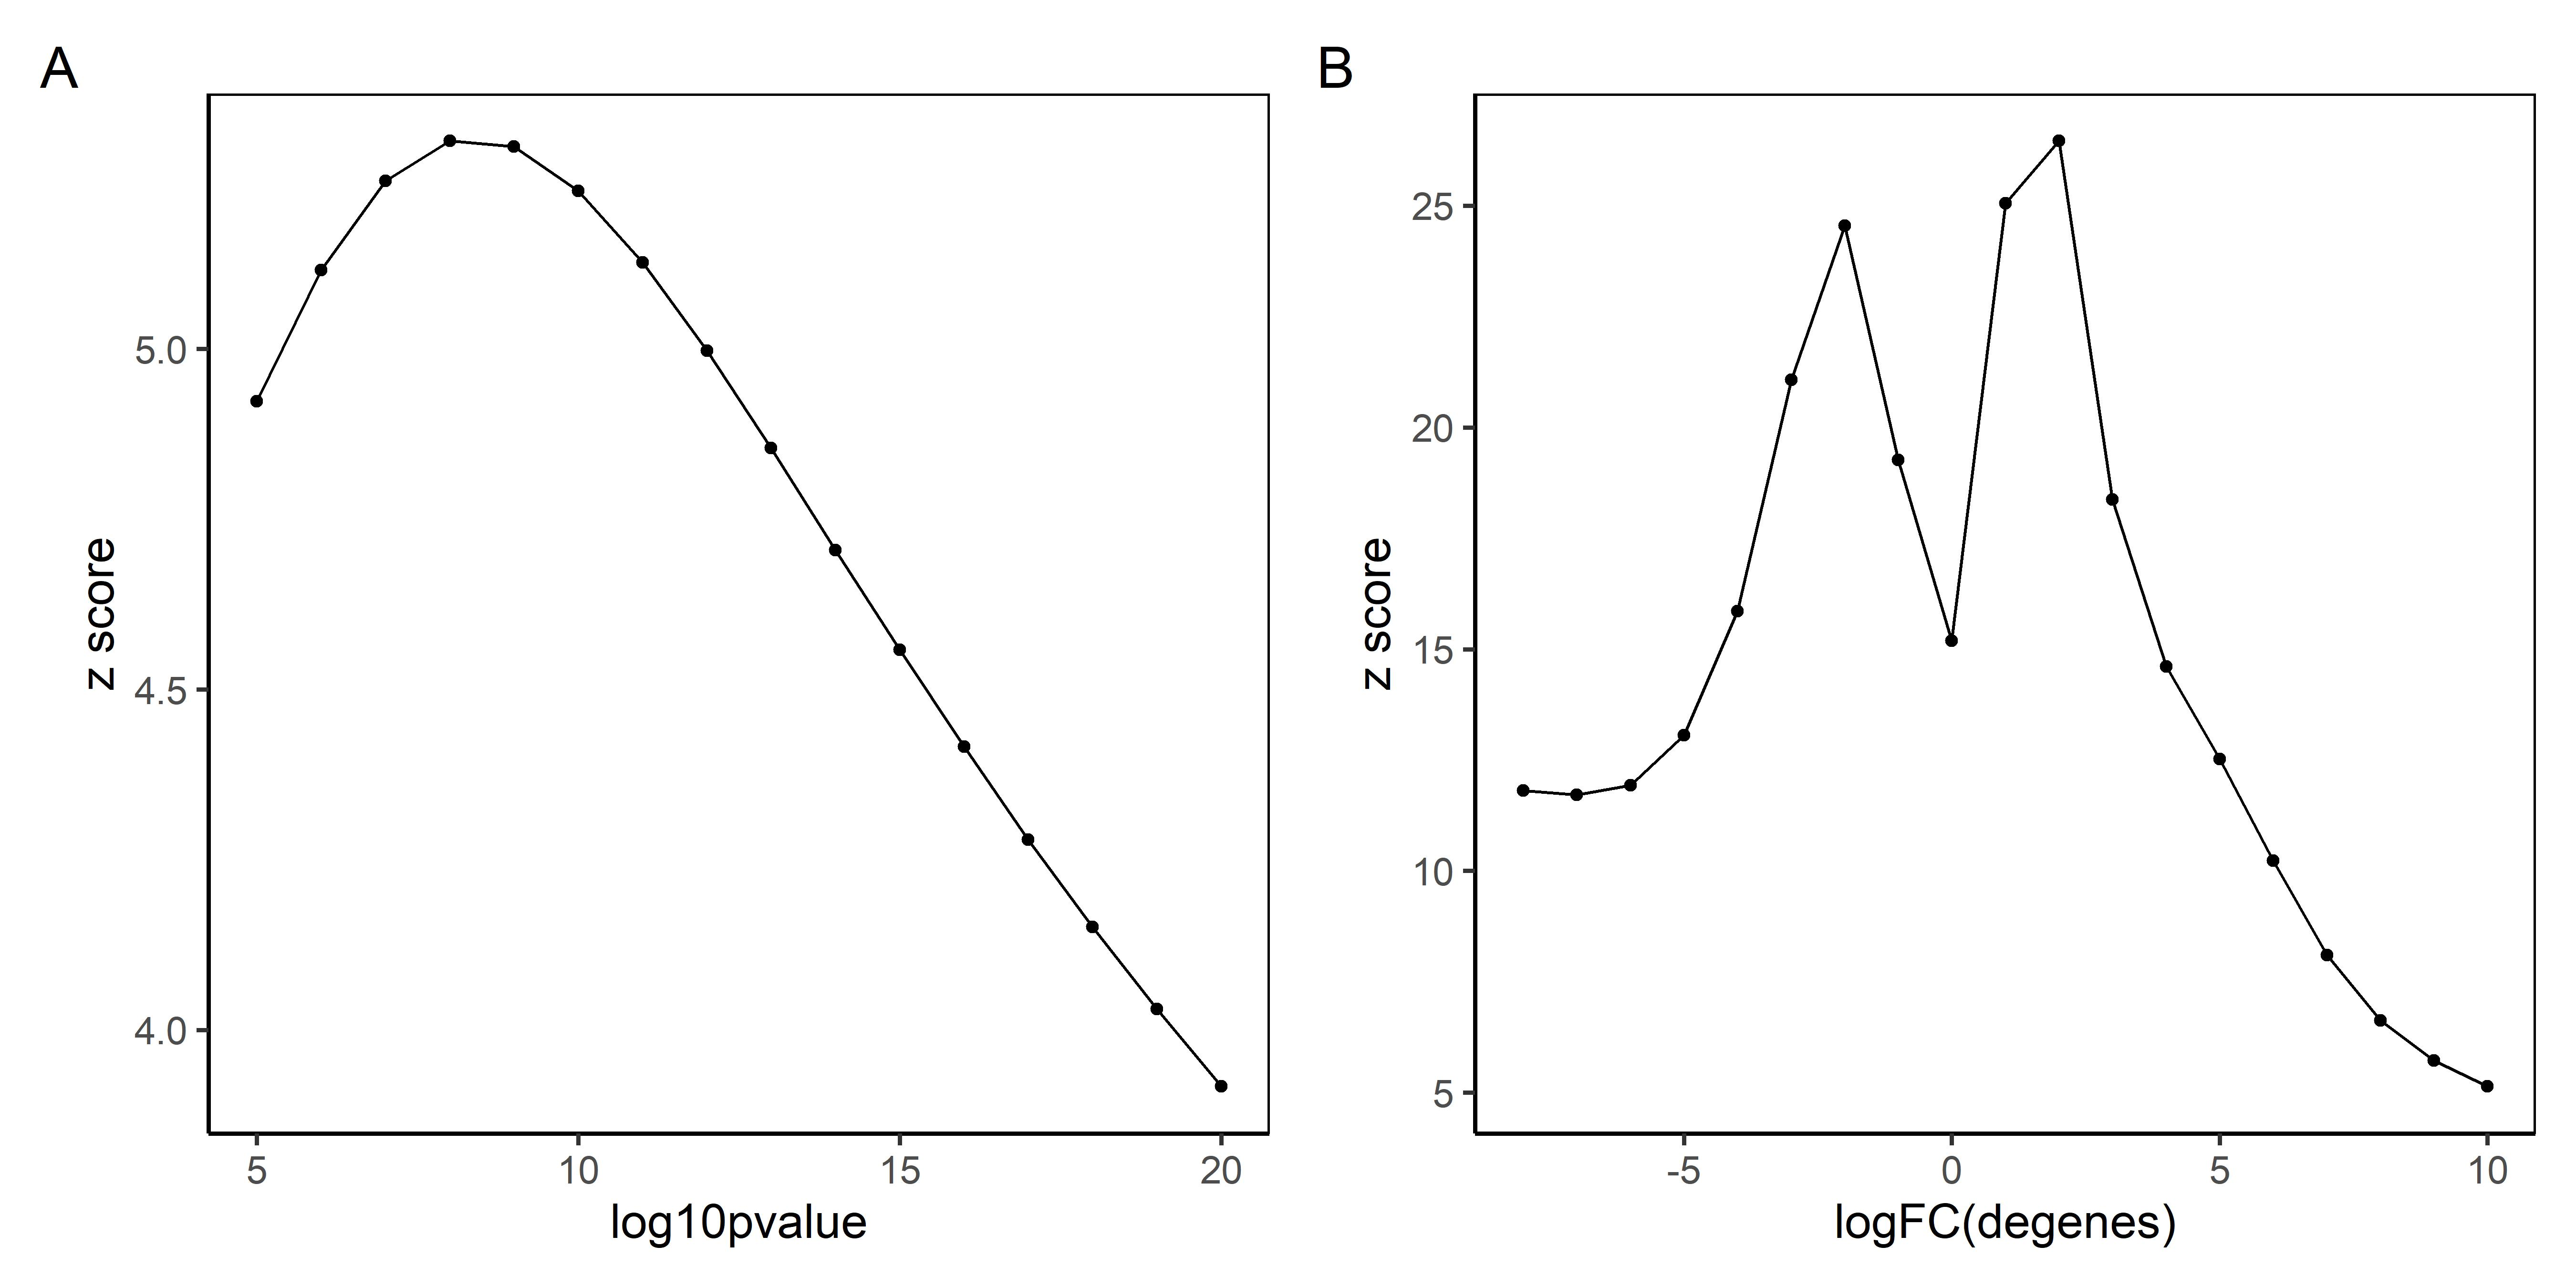
\includegraphics[scale=0.3]{Figures/zscore.jpeg}
\caption{
  $z$ scores against thresholds for liver ATAC-seq and macrophage experiments.
%  The $z$ scores indicated the distance of the observed overlap
%  statistics in terms of standard deviations from the 
%  bootstrap distribution of the overlap count ($R = 1,000$).
  A) \textit{z} score against SNPs -log10 (\textit{p}-value)  in the liver
  dataset. The penalized splines was fitted on the top 1800 SNPs and was used to predict the overlap rate for the -log10 (\textit{p}-value) falling into the range (5,20) with 1 as increment for both observed and null sets data. Then, $z$ scores, indicating the distance of the predicted overlap rate between the observed set and
null sets($R = 1,000$) in terms of SD, was derived. B) \textit{z} score against gene expression logFC of the
  macrophage dataset. The penalized splines was fitted on all DE genes and was used to predict the overlap count for the logFC falling into the range (-8,10) with 1 as increment for both observed and null sets data. Then, $z$ scores, indicating the distance of the predicted overlap count between the observed set and
null sets($R = 1,000$) in terms of SD, was derived.}
\label{fig:suppfig2}
\end{figure*}

\begin{figure*}[htbp]
\centering
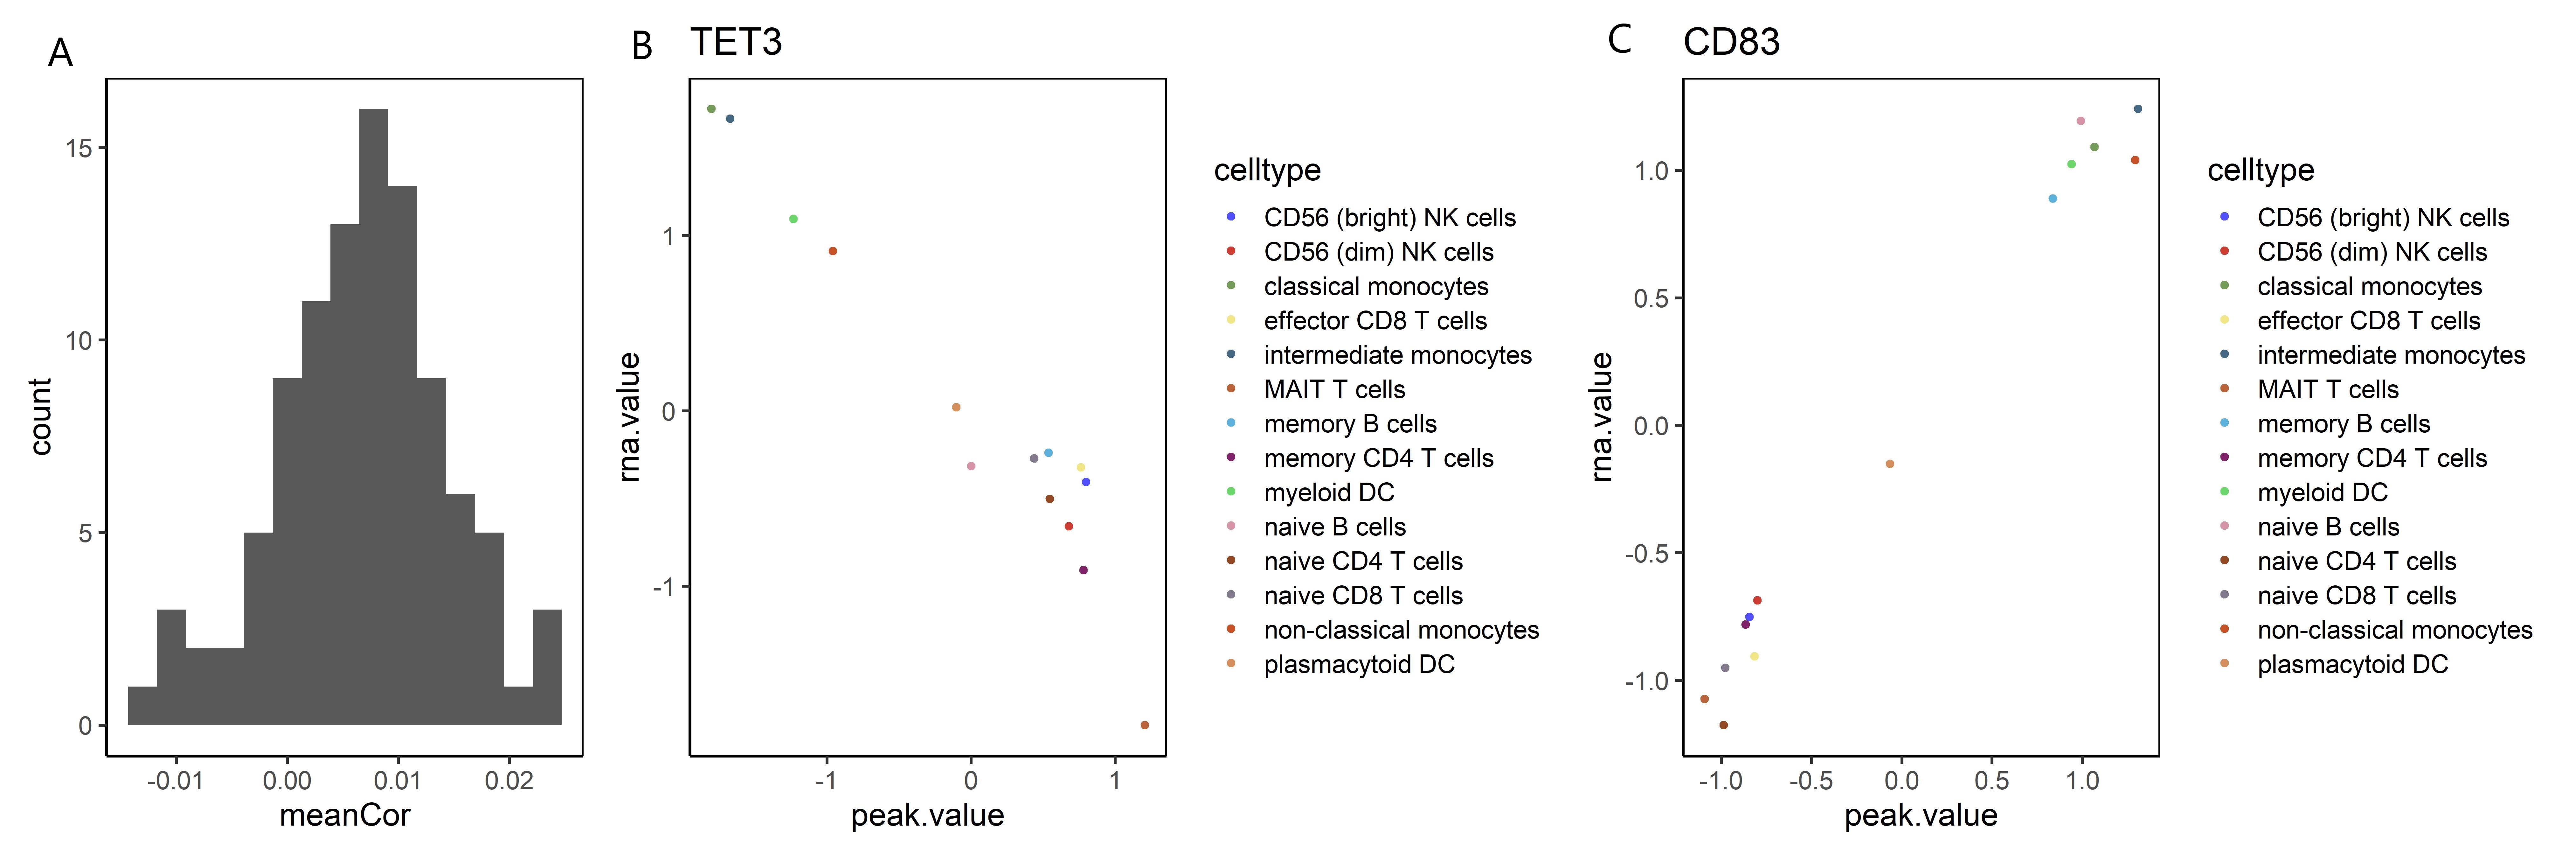
\includegraphics[scale=0.08]{Figures/sfig2.jpeg}
\caption{Correlation analysis of Chromium Single Cell
  Multiome ATAC + Gene Expression dataset. A) The distribution of mean
  correlation of gene expression with bootstrapped
  ATAC-seq peaks and their read counts ($R = 100$).
  B) TET3 read counts (``rna value'') over peak
  chr2:74000098-74003475 read counts (``peak value''),
  colored by cell type. TET3 had
  the most negative observed correlation $\rho = −0.963$.
  C) CD83 read
  counts over peak chr6:14116971-14139988 read counts, colored by cell
  type. The correlation of this gene-promoter pair was 
  0.992 and was the highest among all the pairs.}
\label{fig:suppfig3}
\end{figure*}

\bibliographystyle{natbib}
%\bibliographystyle{achemnat}
%\bibliographystyle{plainnat}
%\bibliographystyle{abbrv}
%\bibliographystyle{bioinformatics}
%
%\bibliographystyle{plain}
%
\bibliography{document}

\end{document}
